\documentclass[dvisvgm, tikz, border=4pt]{standalone}
\begin{document}
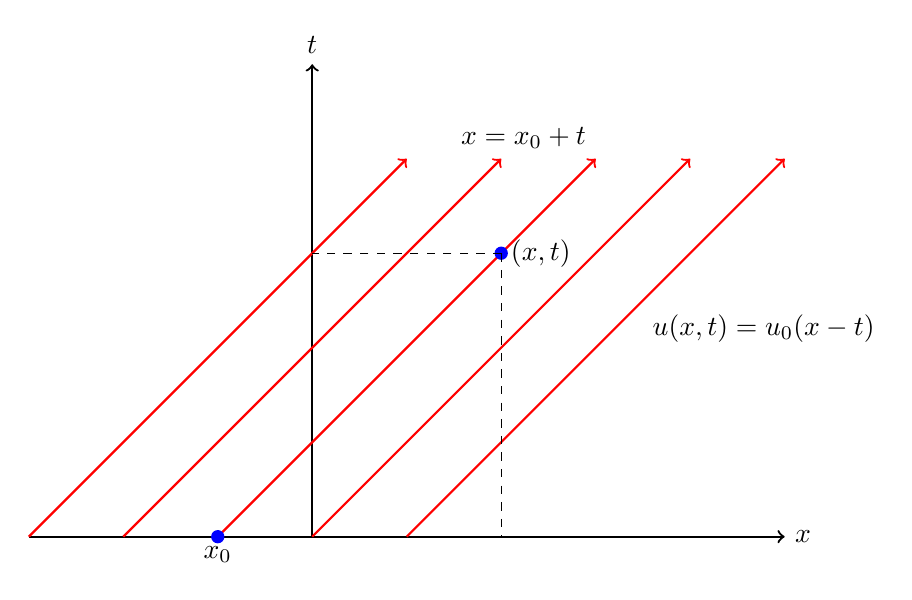
\begin{tikzpicture}[scale=1.2]

\draw[->,thick] (-3,0) -- (5,0) node[right] {$x$};
\draw[->,thick] (0,0) -- (0,5) node[above] {$t$};

\draw[red,thick,->] (-3,0) -- (1,4);
\draw[red,thick,->] (-2,0) -- (2,4);
\draw[red,thick,->] (-1,0) -- (3,4);
\draw[red,thick,->] (0,0) -- (4,4);
\draw[red,thick,->] (1,0) -- (5,4);

\fill[blue] (-1,0) circle (2pt);
\node[below] at (-1,0) {$x_0$};

\fill[blue] (2,3) circle (2pt);
\node[right] at (2,3) {$(x,t)$};

\draw[dashed] (2,3) -- (2,0);
\draw[dashed] (2,3) -- (0,3);

\node[above left] at (3,4) {$x=x_0+t$};
\node[right] at (3.5,2.2) {$u(x,t)=u_0(x-t)$};

\end{tikzpicture}
\end{document}
